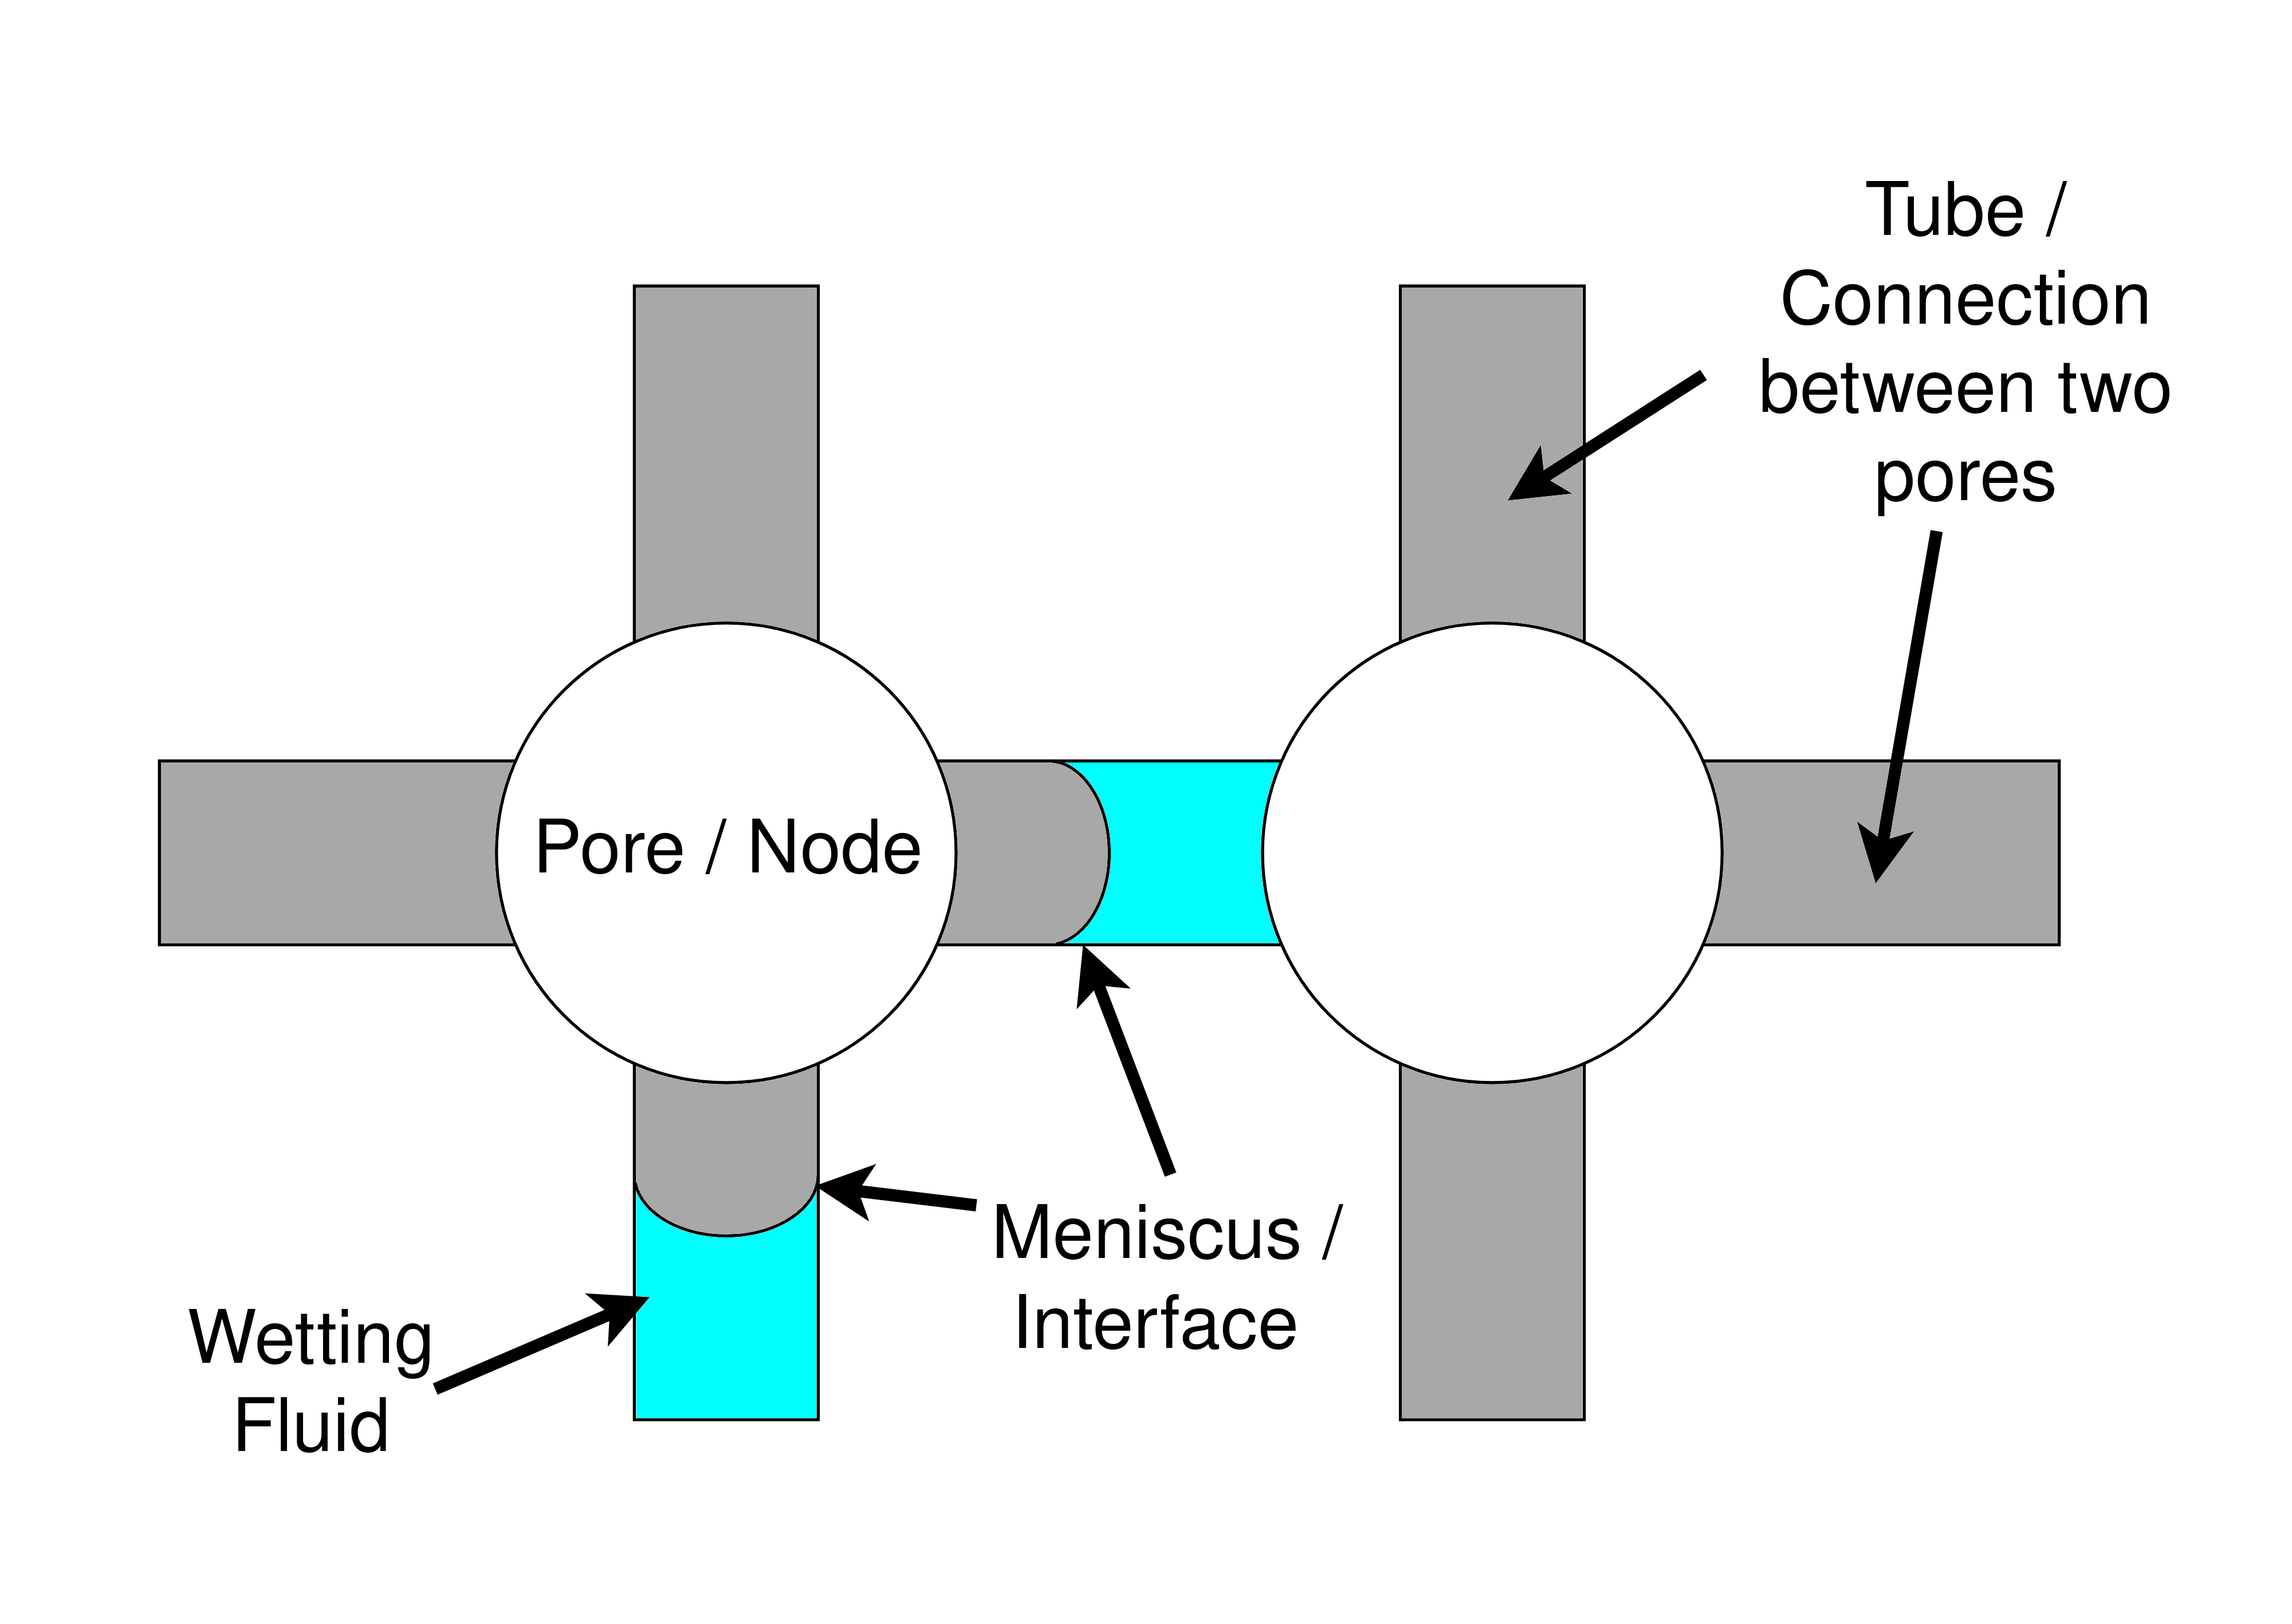
\includegraphics[height=6cm]{fig_descp-of-model}

Figure showing two nodes from the network where the size of the node is much larger than the radius such that the capillary force tends to zero when the meniscus enters a node. In our model the volume of the pore is not taken into consideration. And all the capillaries which are denoted as tubes are cylindrical. All tubes are of equal length for simplicity.

\subsection{Numbering tubes and other parameters in the network model}
	\begin{figure}[H]
		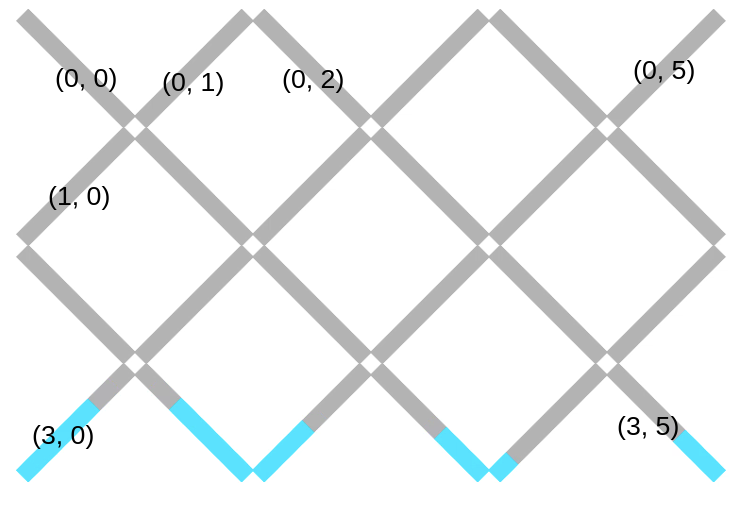
\includegraphics[height=6cm]{fig_numbering-of-ij-tube}
		\caption{Numbering of tubes for a (rows, cols) = (4, 6) network model}
		\label{fig_numbering-of-ij-tube}
	\end{figure}
	
	If $X$ is a parameter then $X_{ij}$ is on the $i$ th row and $j$ th column, note that counting begins from zero. This type of counting is suitable for std::vector< data structure in C++. 
	
\subsection{Linear equations for simple displacement}
	In our model a node is connected to 4 tubes, or less if the node is located at the edges or a corner. The two-dimensional model can be extended to a three-dimensional case similar to \cite{sinha2017effective}.
	
	When generating the linear equations. For each row it is necessary to do the following for each direction:
	
	\[ [P_i] = [P_i] + R_{ij}K_{ij} \]
	\[ [P_j] = [P_j] - R_{ij}K_{ij} \]
	\[ [const] = [const] - 2s_{ij}\sigma K_{ij} \]
	
	Here let $K_{ij} = R^3_{ij}/{M}_{ij}$.

	For simplicity we rewrite the system of four equations as 
	
	In case of 5 nodes in our system, where the pressure of the bottom and top nodes are given and fixed, the matrix for Gaussian elimination will be:

	\[ 
	\begin{pmatrix}
		1 & 0 & 0 & 0 & 0 & P_{up}\\
		0 & 1 & 0 & 0 & 0 & P_{up}\\
		-R_{31}K_{31} & -R_{32}K_{32} & (R_{3k}K_{3k} + ...) & -R_{34}K_{34} & -R_{35}K_{35} & -2\sigma(s_{3k}K_{3k} + ...)\\
		0 & 0 & 0 & 1 & 0 & P_{down}\\
		0 & 0 & 0 & 0 & 1 & P_{down}
	\end{pmatrix}
	\]
	 It can be proven that this matrix always has a solution. Once the solution is determined the flow rate can be calculated using equation \ref{eq:flow-rate-main}, and the velocity of flow in each tube is given by
	 
	\begin{equation} \label{eq:velocity-in-tube}
		\boxed{v_{ij} = \frac{R_{ij}}{8lM_{ij}}(R_{ij}\Delta P_{ij} + 2s_{ij}\sigma)}
	\end{equation}

	
\subsection{Linear equations in case of infinitely many solutions}
	It is possible to calculate the pressures at each node, if the pressures are known on the edges. However when we want to model imhibition, the boundaries are closed and the total volume of a phase remains the same.
	
	\begin{figure}[H]
		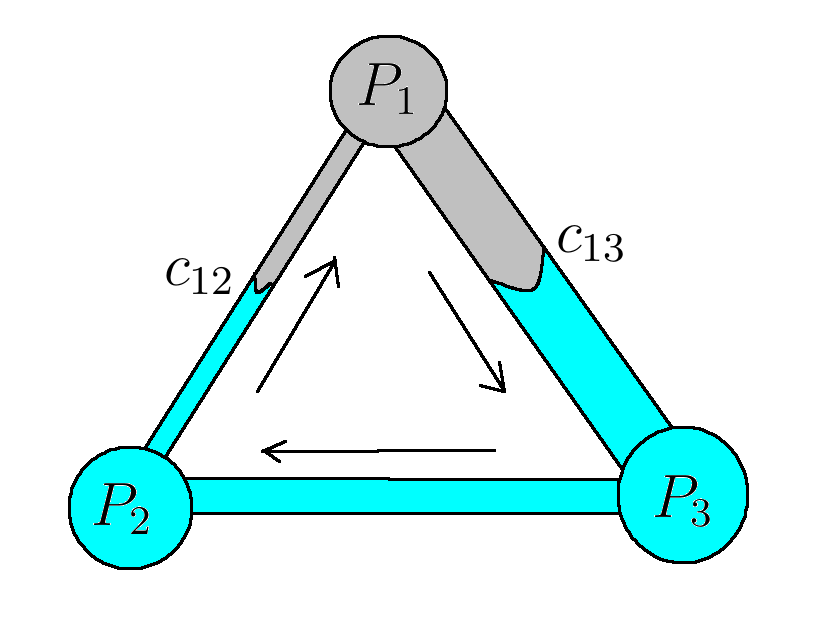
\includegraphics[height=6cm]{fig_zero-linearequation}
		\caption{Case of of infinitely many solutions}
	\end{figure}
	
	Let the flow rates be given by:
	\begin{equation}
		q_{ij} = k_{ij} \Delta P + c_{ij}
	\end{equation}
	
	For $N_{1}$:
	\[ q_{12} = k_{12}(P_1 - P_2) + c_{12} \]
	\[ q_{13} = k_{13}(P_1 - P_3) + c_{13} \]
	
	Since:
	\[ q_{12} + q_{13} = 0 \]
	\[(k_{12} + k_{13})P_1 - k_{12}P_2 - k_{13}P_3 = -c_{12} - c_{13} \]
	
	Then for each node we obtain the following matrix:
	
	\[ 
	\begin{pmatrix}
		(k_{12} + k_{13}) & -k_{12} & -k_{13} & -c_{12} - c_{13} \\
		-k_{21} & (k_{21} + k_{23}) & -k_{23} & -c_{21} - c_{23} \\
		-k_{31} & -k_{32} & (k_{31} + k_{32}) & -c_{31} - c_{32} \\
	\end{pmatrix}
	\]
	
	Note that:
	\[ k_{ij} = k_{ji} \]
	\[ c_{ij} = -c_{ji} \]
	
	Hence the sum of each column of this matrix is zero.
	
	By $R_3 = R_3 + R_1 + R_2$:
	
	\[ 
	\begin{pmatrix}
		(k_{12} + k_{13}) & -k_{12} & -k_{13} & -c_{12} - c_{13} \\
		-k_{21} & (k_{21} + k_{23}) & -k_{23} & -c_{21} - c_{23} \\
		0 & 0 & 0 & 0 \\
	\end{pmatrix}
	\]
	
	This is solved by adding a constant $a$ to one of the column of the matrix for each rows. In our model the centre was chosen to be the zero of pressure. Changing this point does not change the flow rates or the nature of flows.
	
	\[ 
	\begin{pmatrix}
		(k_{12} + k_{13}) & -k_{12} & -k_{13} + a & -c_{12} - c_{13} \\
		-k_{21} & (k_{21} + k_{23}) & -k_{23} + a & -c_{21} - c_{23} \\
		-k_{31} & -k_{32} & (k_{31} + k_{32}) + a & -c_{31} - c_{32} \\
	\end{pmatrix}
	\]
	
	After $R_3 = R_3 + R_1 + R_2$:
	\[ 
	\begin{pmatrix}
		(k_{12} + k_{13}) & -k_{12} & -k_{13} + a & -c_{12} - c_{13} \\
		-k_{21} & (k_{21} + k_{23}) & -k_{23} + a & -c_{21} - c_{23} \\
		0 & 0 & 3a & 0 \\
	\end{pmatrix}
	\]
	
	\[3aP_3 = 0 \]
	
	The solutions exists only if $P_3 = 0$.
	
\subsection{Distribution and recombination}
	The novelty of our model is how we distribute phases in the nodes. When more than two phases flow into a node, the wetting fluid first enters the tube with the thinner radius. Our data structure was constrained to only allow the case for a maximum of two meniscus in a tube.
	
	\begin{figure}[H]
		\centering
		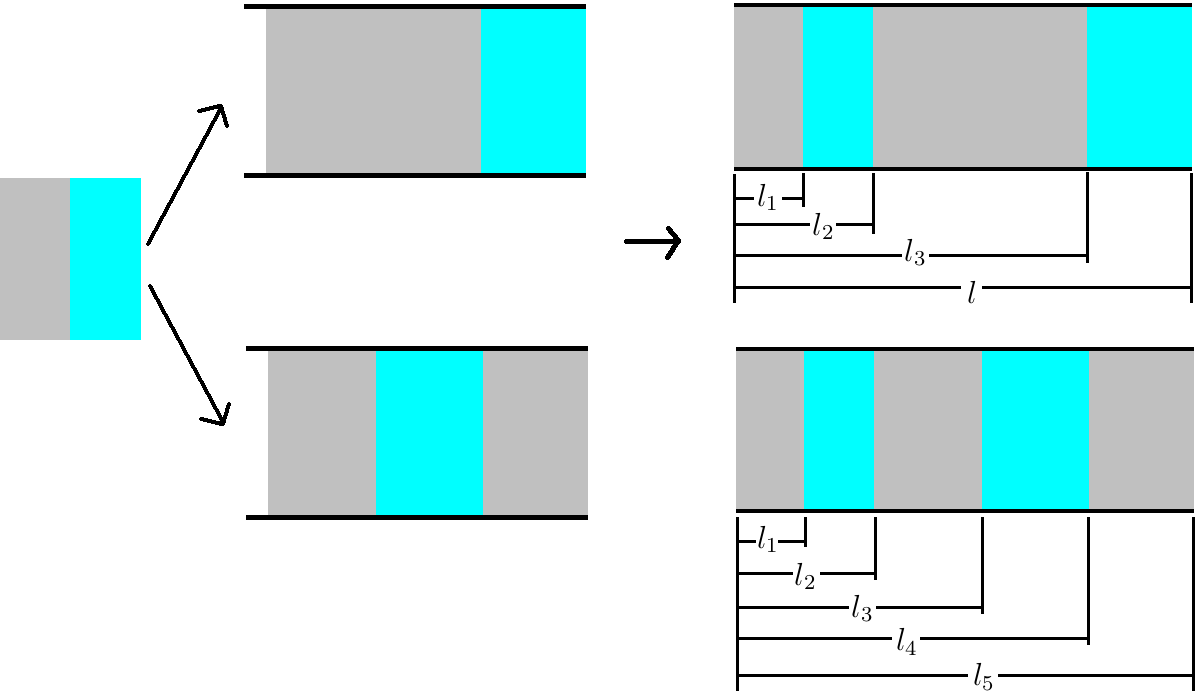
\includegraphics[height=8cm]{fig_center-of-mass}
		\caption{Case of more than two meniscus in a tube}
	\end{figure}
	
	Grey:
	$m_1 = l_1$ at $d_1 = \frac{l_1}{2}$,
	
	$m_2 = l_3 - l_2$ at $d_2 = \frac{(l_3 + l_2)}{2}$
	
	\[m = m_1 + m_2\]
	\[ c_{grey} = \frac{m_1 d_1 + m_2 d_2}{m} \]
	
	\[l_4 = c_{grey} - \frac{m}{2}\]
	\[l_5 = l_4 + m\]
	



\subsection{Algorithm for computation}
	\begin{enumerate}
		\item \textbf{Input Files:} read input files, radius.txt and mns.txt, mns.txt contains the initial setup of the meniscus
		\item \textbf{Random radius:} add very small random values to the radius, this is done in order to remove the case of two equal radius for simplicity, can be removed later
		\item \textbf{Loop time:} do until a certain proportion of invading fluid is reached for example 0.90 or a fixed number of frames:
		
		\begin{enumerate}
			\item \textbf{Pressure:} determine the pressure at each node using the linear equations given in section \ref{sec:linear-equ}.
			\item \textbf{Velocity:} Calculate the velocity using equation \ref{eq:velocity-in-tube} 
			\item \textbf{time step:} determine the time step, it is the $\Delta t = min{l/v{i}}$.
			\item \textbf{volume:} The volume displaced in each tube is determined by iterating through all the tubes, $V_{ij} = v_{ij} * t_{min}$.
			\item \textbf{integration:} 
				\begin{enumerate}
				\item \textbf{Store insertion:} create a matrix to store how much of which fluid to insert in each of these tubes.
				\item \textbf{Loop nodes:} Iterate through all the nodes, and for each of the nodes. 
					\begin{enumerate}
						\item divide the tubes into two categories, flow-in-tube - here the fluid from these tubes flow into the nodes, flow-out-tubes here we insert the fluid into the tube from the node
						\item Find out the total of fluid1, fluid2, which is the total of each fliud from all flow-in-tubes.
						\item Start filling the each of the flow-out-tubes where the flow will go into in ascending order of the radius of the tube. This will be done simply be adding the quantity of fluid1 and fluid2 to the matrix created above.
						\item while filling fist use fluid1, once fluid1 is used up then start using fluid2, which means if in a tube we have to insert two fluids, then fluid1 will go in first.
					\end{enumerate}
				\item \textbf{Fluid addition:} For each of the tubes, add the volume of fluid determined to be added. After addition if there are more than 2 meniscus, then merge them retaining their center of masses.
				\end{enumerate}
			\item \textbf{Picture:} Save a picture of the current configuration.
			\end{enumerate}
		\item {Video:} Make a video file from the pictures.
	\end{enumerate}

\subsection{Possible Cases of Errors}

	\subsubsection{Initial configuration for flow to start}

	The flow did not start when all the meniscus were located inside the nodes. Because in our model we assumed that there is not capillary pressure in the nodes. To overcome this, the meniscus were made to be situated inside the tubes.

	\subsubsection{Case of all meniscus located in the thick tubes}

	The solution of linear equation were such that, the capillary force balanced out the pressure gradient. The pressure was much higher outside in the thick tubes than in the thin tubes. Whether this was caused by error in the process of solving the linear equation or due to the initial setup, needs to be checked again. Error is, that it is impossible to determine whether the coefficient during the process of gauss elimination is zero or not. Because of the way how floating point numbers are handled by the CPU, 0 is often seen as a small number.

\subsection{Simple tests for our model}
	\subsubsection{Filtration}
		\begin{figure}[H]
			\centering
			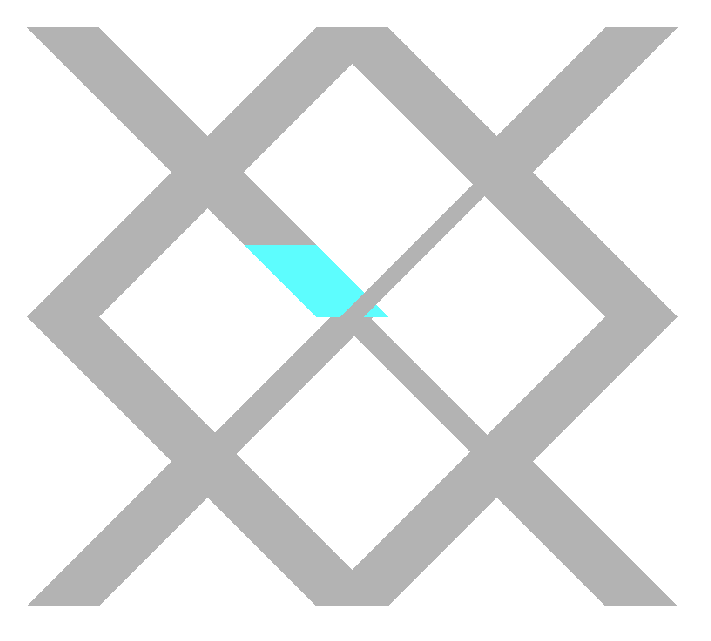
\includegraphics[width=8cm]{fig_test_dist_th01}
			\caption{Initial position of wetting fluid}
		\end{figure}

		\begin{figure}[H]
			\centering
			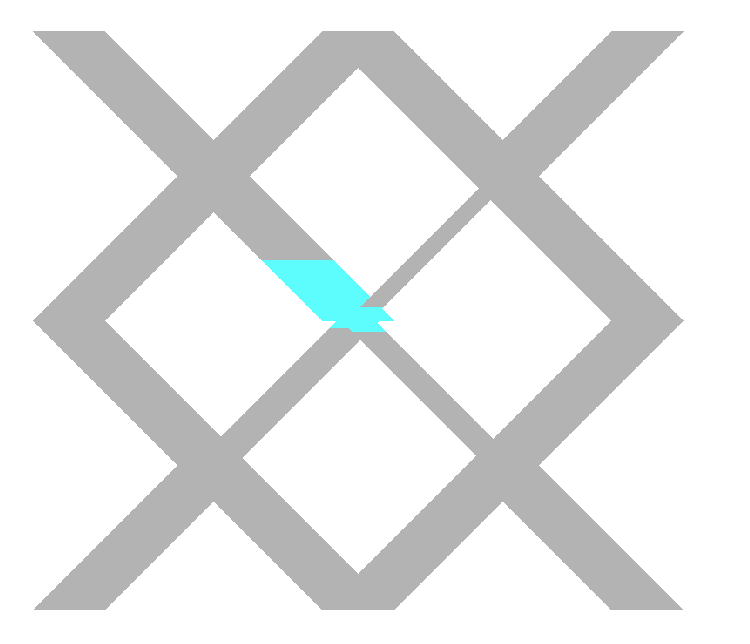
\includegraphics[width=8cm]{fig_test_dist_th02}
			\caption{The wetting fluid chose to move to the tubes with thinner radius.}
			
		\end{figure}
		
		\begin{figure}[H]
			\centering
			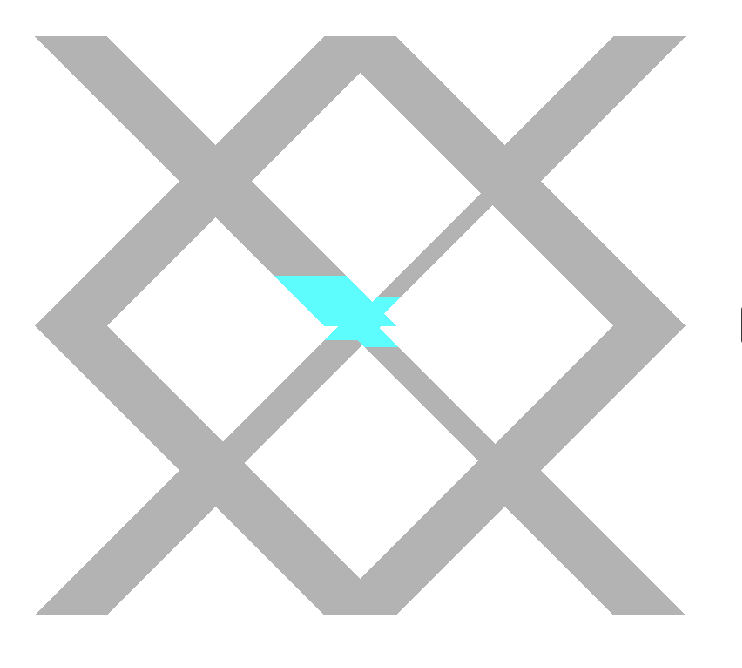
\includegraphics[width=8cm]{fig_test_dist_th03}
			\caption{The flow accelerates as more fluid is in the thinner radius, here viscosity of the wetting fluid is higher.}
		\end{figure}

		\begin{figure}[H]
			\centering
			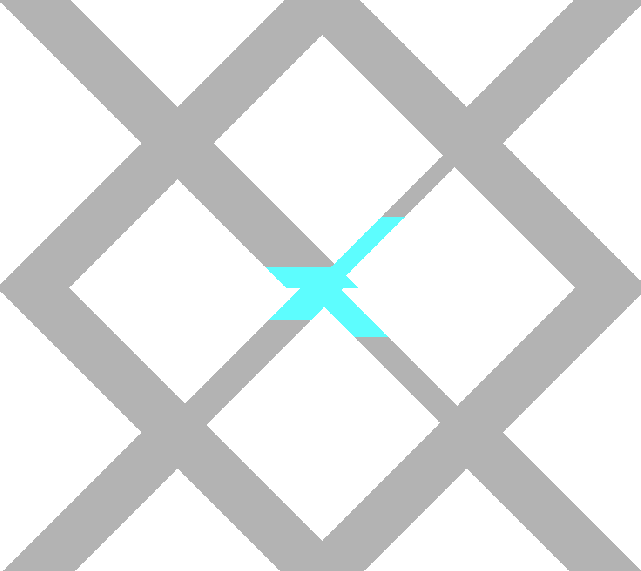
\includegraphics[width=8cm]{fig_test_dist_th04}
			\caption{}
		\end{figure}
		
		\begin{figure}[H]
			\centering
			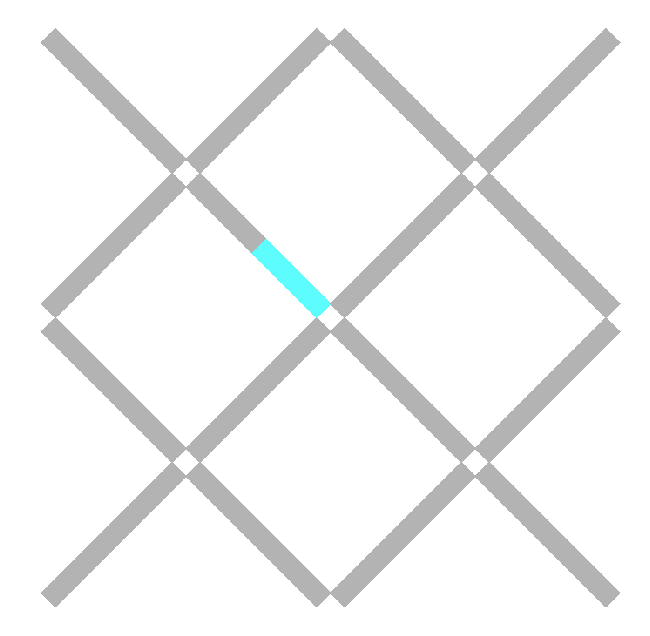
\includegraphics[width=8cm]{fig_test_dist_tn01}
			\caption{The same flow without plotting the radius thickness for clarity.}
		\end{figure}

		\begin{figure}[H]
			\centering
			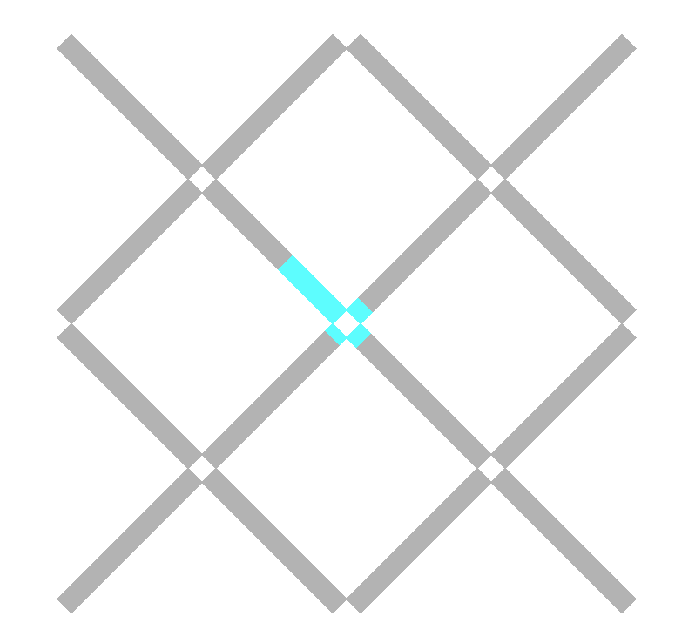
\includegraphics[width=8cm]{fig_test_dist_tn02}
			\caption{}
			
		\end{figure}
		
		\begin{figure}[H]
			\centering
			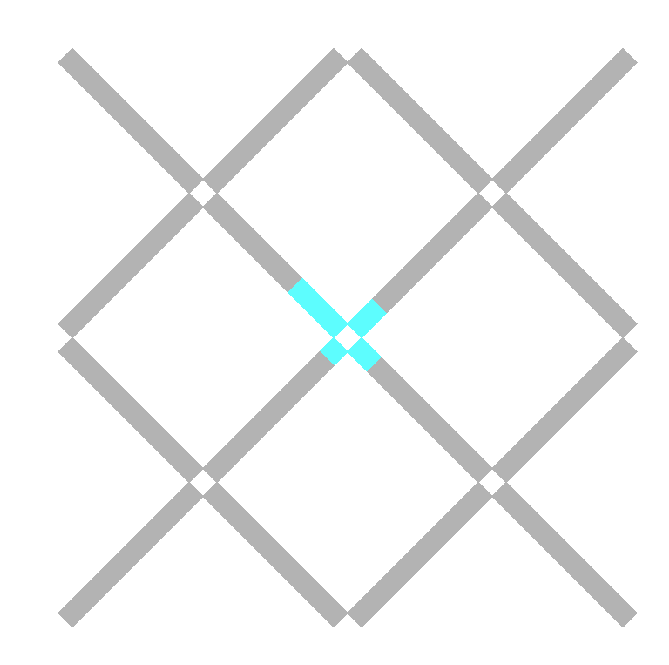
\includegraphics[width=8cm]{fig_test_dist_tn03}
			\caption{}
		\end{figure}

		\begin{figure}[H]
			\centering
			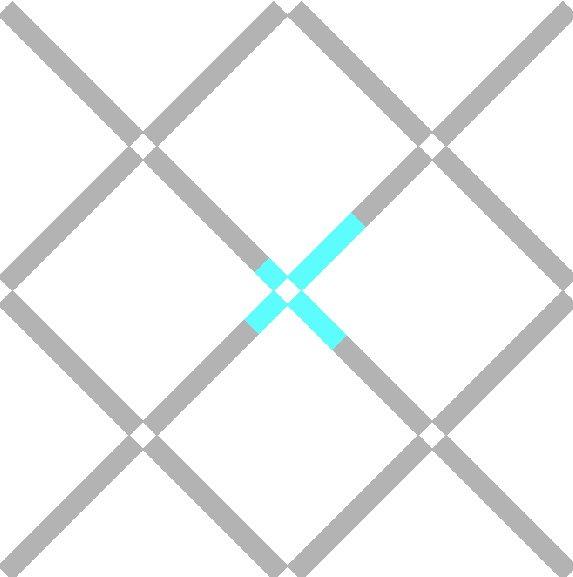
\includegraphics[width=8cm]{fig_test_dist_tn04}
			\caption{}
		\end{figure}
		
		
	\subsubsection{Displacement}
		\begin{figure}[H]
			\centering
			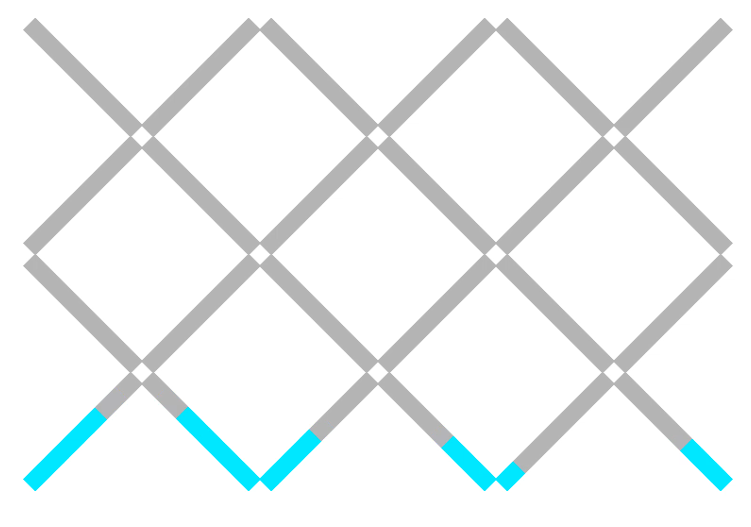
\includegraphics[width=8cm]{fig_initial-fill-distribution}
			\caption{Our model is initially set up such that the wetting fluid is low in saturation and is confined to the bottom of our network. A higher pressure is fixed for all nodes at the bottom layer, while a  low pressure is fixed for the top row.}
			\label{fig_plot-sat-vs-time-disp-one}
		\end{figure}

		\begin{figure}[H]
			\centering
			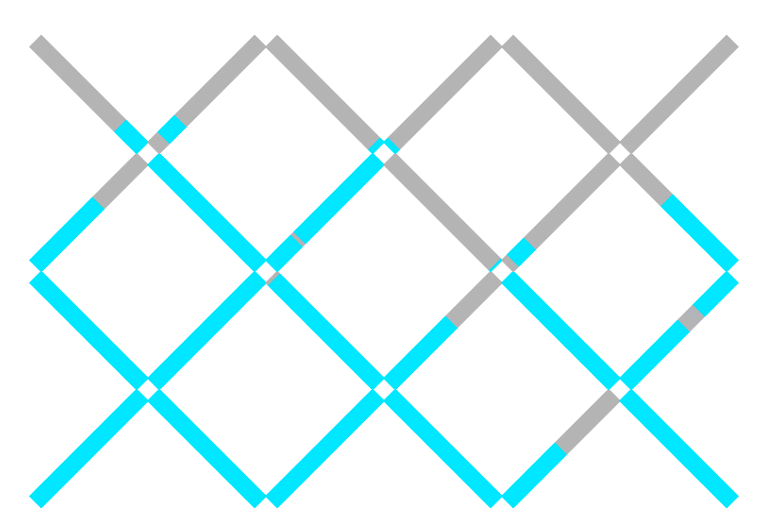
\includegraphics[width=8cm]{fig_final-fill-distribution}
			\caption{In all nodes, law of conservation of volume is applied, since mass is conserved and the phases are non-compressible. However for the bottom layer of nodes, the wetting fluid is injected as much required according to the sum of flow rates determined in the tubes connected to those nodes, while from the top layer of nodes a fluid is removed.}
			\label{fig_plot-sat-vs-time-disp-two}
		\end{figure}
 
	
